\documentclass[a4paper,12pt]{article}

\RequirePackage{epsfig}

\setlength\hoffset{-0.5in}      %% these work quite well with a 12pt font
\setlength\voffset{-0.5in}
\setlength{\textwidth}{6.30in}
\setlength{\textheight}{9.0in}

\bibliographystyle{unsrt}

\begin{document}

\begin{center}
{\Large\bf{Towards Evaluating Creativity in Language}} \\
      \vspace{5.0mm}
{\Large\bf{Project Plan}} \\
      \vspace{8mm}
      {\large\bf{Matey Krastev}}  \\
      \vspace{5.0mm}
       {\tt m.krastev.19@abdn.ac.uk} \\
      \vspace{5.0mm}
      {\em Department of Computing Science,\\
       University of Aberdeen, Aberdeen AB24 3UE, UK} 
\end{center}


\section*{Introduction}

This section should briefly describe the background to your
project and explain why your project is a worthwhile task.
You could add some references here, if appropriate, to cite 
relevant articles
\cite{wooldridge2002,shoham95} and \cite{garcia-camino2005}.

\section*{Goals}

This section should describe the main goals of your project.
In other words, describe \emph{wht} it is that you want to do.
Are you building a tool or an application? What functionality 
already exists, and what will you have to do yourself?

Try to make it clear which goals are central to your project, and which
might be optional extras. Try to be realistic about making your
goals {\em achievable.}


\section*{Methodology}

This section should describe {\em how} you will conduct
your project. You should explain in general terms
the activities you will be carrying out during your project, such as:
%
\begin{itemize}
\item reading about related work -- either to get ideas on how to
      proceed, or to compare your approach with what was done before;
\item learning a new programming language or API;
\item learning about relevant technologies;
\item developing prototypes to test ideas;
\item testing and debugging early design choices.
\end{itemize}
%
The above examples are purely suggestions. You should try to think
of what would be appropriate for your specific project.

\section*{Resources Required}

You should mention here the hardware and software resources you will
require. Even if it seems obvious that you might only need Java and a PC, 
you should still say so!


\section*{Risk Assessment}

Try to describe possible circumstances (e.g. a particular piece of
technology doesn't work or is too expensive) that might cause
the project to become become infeasible. What would you have to do
or change to recover your project?

\section*{Timetable}

This section should describe the {\em schedule} for your project. 
You should describe the various activities you expect to perform
and their durations, along with any deadlines and deliverables.
It is often useful to collect all of this information in a
{\em Gantt chart}, as shown in Figure~\ref{fig:plan} below:

\begin{figure}[htb]
\begin{center}
% \includegraphics[scale=0.65]{ProjectPlan.eps}
\caption{Main Project Activities\label{fig:plan}}
\end{center}
\end{figure}

% For information, this figure was created using xfig, and 
% converted to encapsulated postscript by a command in the Makefile
% before being included as a graphic in the \LaTeX document.

Don't forget to add time at the end of your project for 
evaluation and writing-up! This could easily require 2-3 weeks.


\bibliography{ProjectPlan}

\end{document}
